\subsubsection*{4.(1)}
ダイオードブリッジの両端の電圧を$v_D$,サイリスタブリッジの両端の電圧を$v_T$とする.
このとき$e_d=v_D+v_T$である,
$i_d$が連続して流れていることから消弧角は0である.
したがって$\alpha=\pi/6$のとき$v_D$, $v_T$及び$e_d$は図\ref{fig:4-1-wave}のような波形になる.
以上から電圧の平均は
\begin{align*}
  E_d&=\frac{1}{2\pi}\int_0^{2\pi}e_d dx\\
  &=\frac{2\sqrt{2}V}{\pi}\int_{\pi/6}^\pi\sin xdx\\
  &=\frac{\sqrt{2}V}{\pi}\left(2+\sqrt{3}\right)\simeq336\ \si{\volt}
\end{align*}
また電流の平均は
\begin{align*}
  I_d=\frac{E_d}{R}=6.72\ \si{\ampere}
\end{align*}
となる.
\begin{figure}[htbp]
  \begin{center}
    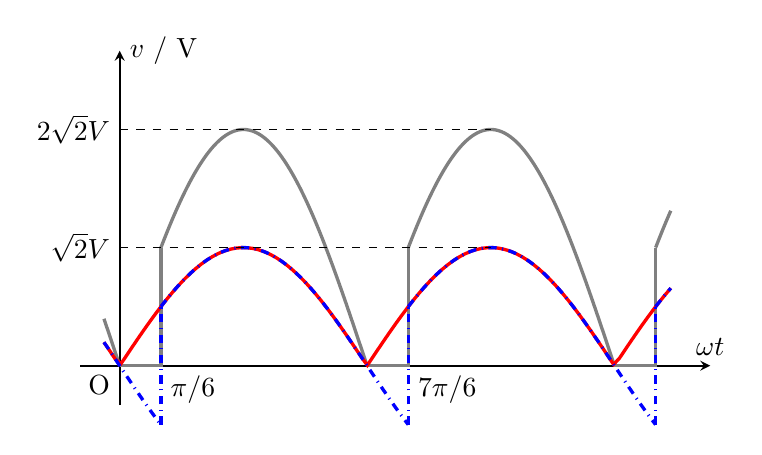
\begin{tikzpicture}
      \draw[->,>=stealth,semithick] (-0.5,0)--(7.5,0)node[above]{$\omega t$}; %x軸
      \draw[->,>=stealth,semithick] (0,-0.5)--(0,4)node[right]{$v$ / V}; %y軸

      \draw[gray,samples=100,very thick,domain=-0.2:0] plot(\x,{-3*sin(\x r)});
      \draw[gray,samples=100,very thick,domain=pi/6:pi*6/6] plot(\x,{3*sin(\x r)});
      \draw[gray,samples=100,very thick,domain=pi*7/6:pi*12/6] plot(\x,{-3*sin(\x r)});
      \draw[gray,samples=100,very thick,domain=pi*13/6:7] plot(\x,{3*sin(\x r)});
      \draw[gray,very thick] (0,0)--(pi/6,0)--(pi/6,1.5);
      \draw[gray,very thick] (pi,0)--(pi*7/6,0)--(pi*7/6,1.5);
      \draw[gray,very thick] (2*pi,0)--(pi*13/6,0)--(pi*13/6,1.5);
      \draw[dashed, thin] (0,3)node[left]{$2\sqrt{2}V$}--(pi*3/2,3);

      \draw[red,samples=100,very thick,domain=-0.2:7] plot(\x,{abs(1.5*sin(\x r))});
      \draw[blue,dash dot,samples=100,very thick,domain=-0.2:pi/6] plot(\x,{-1.5*sin(\x r)});
      \draw[blue,dash dot,very thick] (pi/6,{-1.5*sin(pi/6 r)})--(pi/6,{1.5*sin(pi/6 r)});
      \draw[blue,dash dot,samples=100,very thick,domain=pi/6:pi*7/6] plot(\x,{1.5*sin(\x r)});
      \draw[blue,dash dot,very thick] (pi*7/6,{-1.5*sin(pi/6 r)})--(pi*7/6,{1.5*sin(pi/6 r)});
      \draw[blue,dash dot,samples=100,very thick,domain=pi*7/6:pi*13/6] plot(\x,{-1.5*sin(\x r)});
      \draw[blue,dash dot,very thick] (pi*13/6,{-1.5*sin(pi/6 r)})--(pi*13/6,{1.5*sin(pi/6 r)});
      \draw[blue,dash dot,samples=100,very thick,domain=pi*13/6:7] plot(\x,{1.5*sin(\x r)});
      \draw (0,0)node[below left]{O};
      \draw (pi/6,0)node[below right]{$\pi/6$};
      \draw (pi*7/6,0)node[below right]{$7\pi/6$};
      \draw[dashed, thin] (0,1.5)node[left]{$\sqrt{2}V$}--(pi*3/2,1.5);
    \end{tikzpicture}
  \end{center}
  \caption{波形(赤線:$v_D$,青線:$v_T$,灰線:$v_D+v_T$)}
  \label{fig:4-1-wave}
\end{figure}
\newpage
\subsubsection*{4.(2)}
$\alpha=\pi$のとき波形は図\ref{fig:4-2-wave-1}のようになる.
このとき明らかに
\begin{align*}
  E_d=0
\end{align*}
で最小値を取る.また$\alpha=0$のとき波形は図\ref{fig:4-2-wave-2}のようになる.
このとき$e_d$の平均値は
\begin{align*}
  E_d&=\frac{1}{\pi}\int_0^\pi e_ddx\\
  &=\frac{4\sqrt{2}V}{\pi}\simeq360\ \si{\volt}
\end{align*}
で最大値を取る.
\begin{figure}[htbp]
  \begin{center}
    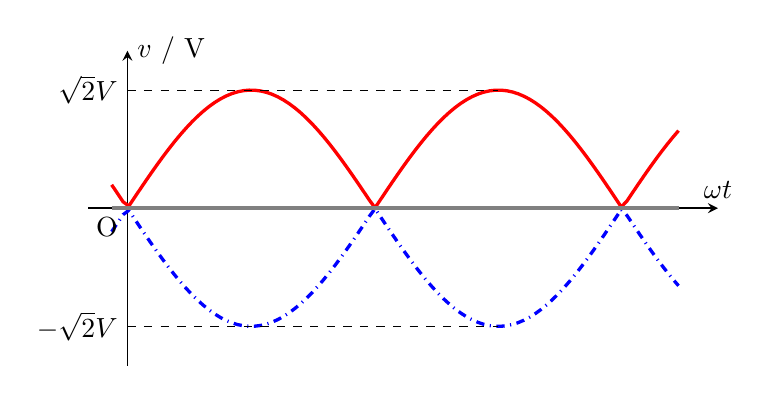
\begin{tikzpicture}
      \draw[->,>=stealth,semithick] (-0.5,0)--(7.5,0)node[above]{$\omega t$}; %x軸
      \draw[->,>=stealth,semithick] (0,-2)--(0,2)node[right]{$v$ / V}; %y軸

      \draw[red,samples=100,very thick,domain=-0.2:7] plot(\x,{abs(1.5*sin(\x r))});
      \draw[blue,dash dot,samples=100,very thick,domain=-0.2:7] plot(\x,{-abs(1.5*sin(\x r))});
      \draw[gray,ultra thick] (-0.2,0)--(7,0);
      \draw[dashed, thin] (0,1.5)node[left]{$\sqrt{2}V$}--(pi*3/2,1.5);
      \draw[dashed, thin] (0,-1.5)node[left]{$-\sqrt{2}V$}--(pi*3/2,-1.5);
      \draw (0,0)node[below left]{O};
    \end{tikzpicture}
  \end{center}
  \caption{最小値の波形(赤線:$v_D$,青線:$v_T$,灰線:$v_D+v_T$)}
  \label{fig:4-2-wave-1}
\end{figure}
\begin{figure}[htbp]
  \begin{center}
    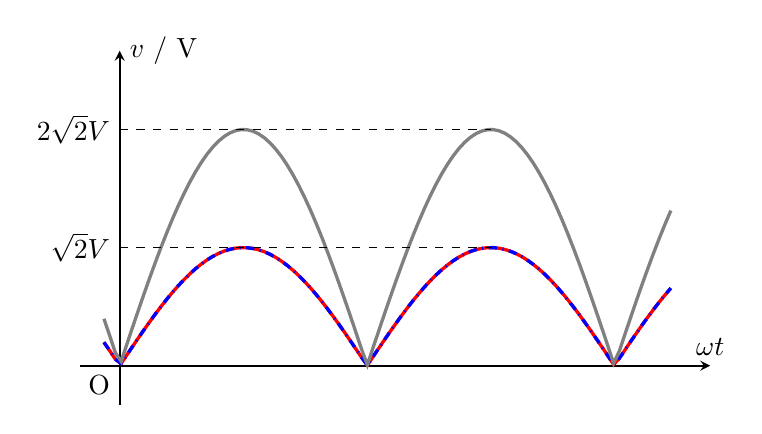
\begin{tikzpicture}
      \draw[->,>=stealth,semithick] (-0.5,0)--(7.5,0)node[above]{$\omega t$}; %x軸
      \draw[->,>=stealth,semithick] (0,-0.5)--(0,4)node[right]{$v$ / V}; %y軸

      \draw[red,samples=100,very thick,domain=-0.2:7] plot(\x,{abs(1.5*sin(\x r))});
      \draw[blue,dash dot,samples=100,very thick,domain=-0.2:7] plot(\x,{abs(1.5*sin(\x r))});
      \draw[gray,samples=100,very thick,domain=-0.2:7] plot(\x,{abs(3*sin(\x r))});
      \draw[dashed, thin] (0,1.5)node[left]{$\sqrt{2}V$}--(pi*3/2,1.5);
      \draw[dashed, thin] (0,3)node[left]{$2\sqrt{2}V$}--(pi*3/2,3);
      \draw (0,0)node[below left]{O};
    \end{tikzpicture}
  \end{center}
  \caption{最大値の波形(赤線:$v_D$,青線:$v_T$,灰線:$v_D+v_T$)}
  \label{fig:4-2-wave-2}
\end{figure}